%%%%%%%%%%%%%%%%%%%%%%%%%%%%%%%%%%%%%%%%%%%%%%%%%%%%%%%%%%%%%%%%%%%%%%%%%%%%%%%%%%%
% Thiago Pelizoni
%%%%%%%%%%%%%%%%%%%%%%%%%%%%%%%%%%%%%%%%%%%%%%%%%%%%%%%%%%%%%%%%%%%%%%%%%%%%%%%%%%%
% Pós-graduação em Engenharia de Software - Universidade São Judas Tadeu - São Paulo - SP
%%%%%%%%%%%%%%%%%%%%%%%%%%%%%%%%%%%%%%%%%%%%%%%%%%%%%%%%%%%%%%%%%%%%%%%%%%%%%%%%%%

%%%%%%%%%%%%%%%%%%%%%%%%%%%%%%%%%%%%%%%%%%%%%%%%%%%%%%%%%%%%%%%%%%%%%%%%%%%%%%%%%%%
% Trabalho referente a matéria de Métricas de Software
%%%%%%%%%%%%%%%%%%%%%%%%%%%%%%%%%%%%%%%%%%%%%%%%%%%%%%%%%%%%%%%%%%%%%%%%%%%%%%%%%%%

\documentclass[11pt, a4paper]{article}				

\usepackage[utf8]{inputenc}
\usepackage[brazil]{babel}	
\usepackage{graphicx,color}
\usepackage[left=2.0cm,top=2.5cm,right=2.0cm,bottom=2.0cm]{geometry}
\usepackage{enumerate}
\usepackage{epigraph}
\usepackage{abntcite}
\usepackage{float}

% Título do trabalho
\title{Uso de métricas de software na quantificação dos custos de erros encontrados em um projeto real}

% Autor
\author{
	Thiago Pelizoni \\
	André Terceiro \\
	Rodrigo Raminelli
}

\date{2013}


%%%%%%%%%%%%%%%%%%%%%%%%%%%%%%%%%%%%%%%%%%%%%%%%%%%%%%%%%%%%%%%%%%%%%%%%%%%%%%%%%%%

\begin{document}

% Faz a criação do título do documento
\maketitle

%%%%%%%%%%%%%%%%%%%%%%%%%%%%%%%%%%%%%%%%%%%%%%%%%%%%%%%%%%%%%%%%%%%%%%%%%%%%%%%%%%%
% Resumo
%%%%%%%%%%%%%%%%%%%%%%%%%%%%%%%%%%%%%%%%%%%%%%%%%%%%%%%%%%%%%%%%%%%%%%%%%%%%%%%%%%%
\begin{abstract}
O custo de defeitos em software tende a crescer exponencialmente a medida que as etapas do desenvolvimento de software avançam. O valor pode ser alto ao ponto de custar entre 90 a 880 vezes o valor do levantamento deste requisito na sua fase inicial.\cite[p. 37]{NISL} A Engenharia de Software utiliza métricas de produto afim de construir um software de alta qualidade. Desta forma, este trabalho tem o intuito de demonstrar a aplicação das técnicas de métricas de software no projeto de inscrição dos participantes da Corrida de São Silvestre afim de quantificar os erros encontrados, seja na fase de testes, homologação ou produção e calcular o custo destes erros, evidenciando o quanto a empresa economizaria em uma melhoria no processo.


\end{abstract}


%%%%%%%%%%%%%%%%%%%%%%%%%%%%%%%%%%%%%%%%%%%%%%%%%%%%%%%%%%%%%%%%%%%%%%%%%%%%%%%%%%%
% 1. Introdução
%%%%%%%%%%%%%%%%%%%%%%%%%%%%%%%%%%%%%%%%%%%%%%%%%%%%%%%%%%%%%%%%%%%%%%%%%%%%%%%%%%%
% Descreve porquê o trabalho foi feito.
\section{Introdução}
São comuns abordagens a respeito de qualidade de software, que é necessário seguir boas práticas para se obter um software de alta qualidade, no entanto, como pode ser definida a qualidade? Em um sentido geral, qualidade de software é a satisfação de requisitos funcionais e de desempenho explicitamente declarados, normas de software explicitamente documentadas e características implícitas que são esperadas em todo o software desenvolvido profissionalmente. A partir desta definição, podem ser enfatizados três pontos importantes:

\begin{enumerate}
	\item Requisitos de software são a fundação a partir da qual a qualidade é medida. A falta de conformidade com os requisitos é falta de qualidade.
	\item Normas especificadas definem um conjunto de critérios de desenvolvimento que guiam o modo pelo qual o software é construído. Se os critérios não são seguidos, quase sempre, irá resultar em falta de qualidade.
	\item Há um conjunto de requisitos implícitos que frequentemente não são mencionados, por exemplo, o desejo de facilidade de uso (usabilidade). Se os software satisfaz os requisitos explícitos, mas deixa de satisfazer requisitos implícitos, a qualidade do software é suspeita.
\end{enumerate}
\cite[p.349]{pressman}

\subsection{Métricas de Software}
\epigraph{A qualidade de um produto é função de quanto ele muda o mundo para melhor}{Tom DeMarco\cite[p.350]{pressman}}

Um elemento-chave que a engenharia utiliza em seu processo é a medição, de modo a ter um melhor entendimento dos atributos dos modelos criados afim de avaliar a qualidade seus produtos ou sistemas desenvolvidos.

De acordo com Pressman, a medição é um processo pelo qual números ou símbolos são associados aos atributos de entidades do mundo real, de modo que os determinem de acordo com regras claramente definidas. Nas ciências físicas, medicina, economia e mais recentemente nas ciências sociais, atualmente é possível medir atributos que anteriormente não eram mensuráveis. Obviamente, tais medições em engenharia de software não são tão refinadas quanto muitas medições nas ciências físicas mas, elas existem e decisões importantes são tomadas com base nelas. A obrigação de tentar medir o não mensurável afim de melhorar o entendimento de entidades particulares é tão potente em engenharia de software como em qualquer outra disciplina.\cite[p.348]{pressman}

\subsubsection{Medidas, Métricas e Indicadores}
\epigraph{Uma ciência é tão madura quanto seus instrumentos de medição}{Louis Pasteur\cite[p.352]{pressman}}

Em engenharia de software, uma medida fornece uma indicação quantitativa da extensão, qualidade, dimensão, capacidade ou tamanho de algum produto ou processo, deste modo, podemos definir como \textit{medição} o ato de determinar uma medida.\cite[p.348]{pressman}

Quando um ponto de dados é coletado, por exemplo, o número de erros descoberto em um componente de software, uma medida é estabelecida. Neste caso, a medição ocorre como o resultado da coleção de um ou mais ponto de dados, por exemplo, um certo número de revisões de componentes e testes de unidade são investigados afim de coletar medidas do número de erros de cada um.

Uma métrica de software visa relacionar as medidas individuais de algum modo, por exemplo, o número de erros encontrados por revisão ou o número médio de erros encontrados por teste de unidade. Com posse dessas informações, um engenheiro de software desenvolve métricas de modo que os indicadores possam ser obtidos. Um \textit{indicador} consiste em um \textit{métrica} ou em uma combinação de \textit{métricas} cujo intuito é fornecer uma profundidade na visão do processo de software, projeto de software ou o produto em si.\cite{pressman}

\subsubsection{Princípios de Medição}
De acordo com Pressman um processo de medição pode ser caracterizado por cinco atividades:

\begin{enumerate}
	\item \textit{Formulação}: A derivação de medidas e métricas de software adequadas para a representação do software que está sendo considerado.
	\item \textit{Coleta}: Mecanismo usado para acumular os dados necessários para derivar as métricas formuladas.
	\item \textit{Análise}: Cálculo de métricas e aplicação das ferramentas matemáticas.
	\item \textit{Interpretação}: Avaliação das métricas em um esforço para ganhar profundidade na visão da qualidade da representação.
	\item \textit{Realimentação}: Recomendações derivadas da interpretação das métricas de produto transmitidas à equipe de software.
\end{enumerate}
\cite[p.353]{pressman}

% Mostrar no trabalho o processo e como são feitos os testes e a homologação e como se reportam os erros em teste, homologação e produção. É interessante descrever o processo de inspeção feita ao receber o pull request;

% Qual o valor hora de cada profissional envolvido: testador, programador, "homologador", equipe de suporte (se for envolvida em repassar a informação de um erro em produção, por exemplo) etc. Assim poderemos calcular o custo dos profissionais envolvidos para cada tipo de erro.

% Se você detectar algum outro custo gerado por exemplo por um erro em produção, é interessante mencionar também.

%Ter as informações sobre os erros detectados em produção, homologação e testes;

\subsection{Objetivo deste trabalho}
Tendo por base as informações anteriormente citadas, o objetivo deste trabalho demonstrar a aplicação das técnicas de métricas no projeto de inscrição dos participantes da Corrida de São Silvestre, afim de quantificar os erros encontrados, sejam estes na fase de testes, homologação ou produção; calcular o custo destes erros afim evidenciar o quanto a empresa economizaria em uma melhoria no processo, detectando os erros em fases do processo de desenvolvimento em que tal detecção é menos onerosa em termos financeiros.


%%%%%%%%%%%%%%%%%%%%%%%%%%%%%%%%%%%%%%%%%%%%%%%%%%%%%%%%%%%%%%%%%%%%%%%%%%%%%%%%%%%
% 2. Materiais e métodos – como foi feito?
%%%%%%%%%%%%%%%%%%%%%%%%%%%%%%%%%%%%%%%%%%%%%%%%%%%%%%%%%%%%%%%%%%%%%%%%%%%%%%%%%%%
% – Referencial teórico
\section{Materiais e métodos}
Nesta sessão iremos descrever quais foram as tecnologias utilizadas no desenvolvimento do projeto, o processo de testes e homologação, qual o procedimento utilizado para reportar erros e consertá-los.

\subsection{O projeto}
O projeto ao qual foi estudo de caso descrito neste artigo foi o de inscrição dos participantes da corrida de Sao Silvestre 2013 desenvolvido pela Fundação Casper Líbero. Este serviu como estudo de caso conta com mais de 150.000 linhas de de código. A linguagem de programação utilizada é PHP\footnote{PHP é uma linguagem de programação interpretada, livre, usada originalmente apenas para o desenvolvimento de aplicações server-side, capazes de gerar conteúdo dinâmico na Web.} na versão 5.3.18, Zend Framework 1.12\footnote{Zend Framework é um framework para aplicações Web de código aberto implementado em PHP 5 completamente orientado a objetos,  licenciado sob a New BSD License.}, banco de dados Oracle\footnote{Oracle é um SGBD (sistema gerenciador de banco de dados)}, controlador de versão Git\footnote{Git é um sistema de controle de versão distribuído projetado e desenvolvido por Linus Torvalds.} e o Trello\footnote{Trello é um organizador de tarefas e eventos bastante dinâmico e funcional, bastante utilizado para gerenciar projetos com a metodologia Scrum.} para gerenciamento das atividades.

O projeto citado havia sido criado em 2012 porém, passou por diversas modificações arquiteturais, visuais e melhorias em geral de modo a englobar novas regras de negócio bem como, correções de problemas identificado na versão anterior.

\subsection{Testes}
O projeto não conta com testes unitários. Os testes em sua maioria são efetuado pelos analistas de negócio do produto de maneira manual. Afim automatizar estes testes manuais, uma bateria de testes do sistema foram criados utilizando o Selenium IDE\footnote{Selenium IDE é um ambiente integrado de desenvolvimento para scripts de testes automatizados simulando o comportamento de um usuário.}. Desta forma, a cada nova funcionalidade criada ou, correção efetuada, estes testes são rodados pelo desenvolvedor. Todavia, os responsáveis pela homologação efetuam os testes manualmente.

%AAAAA\cite{melhoria-processo-indicadores}
\subsection{O processo de desenvolvimento}
A empresa não segue uma metodologia de desenvolvimento de mercado, por exemplo, Scrum, RUP, etc. Trata-se de um desenvolvimento incremental onde, cada funcionalidade é especificada, desenvolvida, testada e colocada em produção.

\subsubsection{Board do projeto}

Como dito anteriormente, a empresa utiliza-se do Trello para o gerenciamento das atividades de um projeto. Cada projeto refere-se unica e exclusivamente a um board\footnote{O board de um projeto no Trello é o equivalente a Kanban online, conforme pode ser observado na figura "Board das tarefas do projeto".}, de modo a não misturar informações com outros projetos. Na figura a seguir podemos observar o board do projeto mencionado por este artigo.

\begin{figure}[H]
  \caption{Board das tarefas do projeto}
  \centering 
  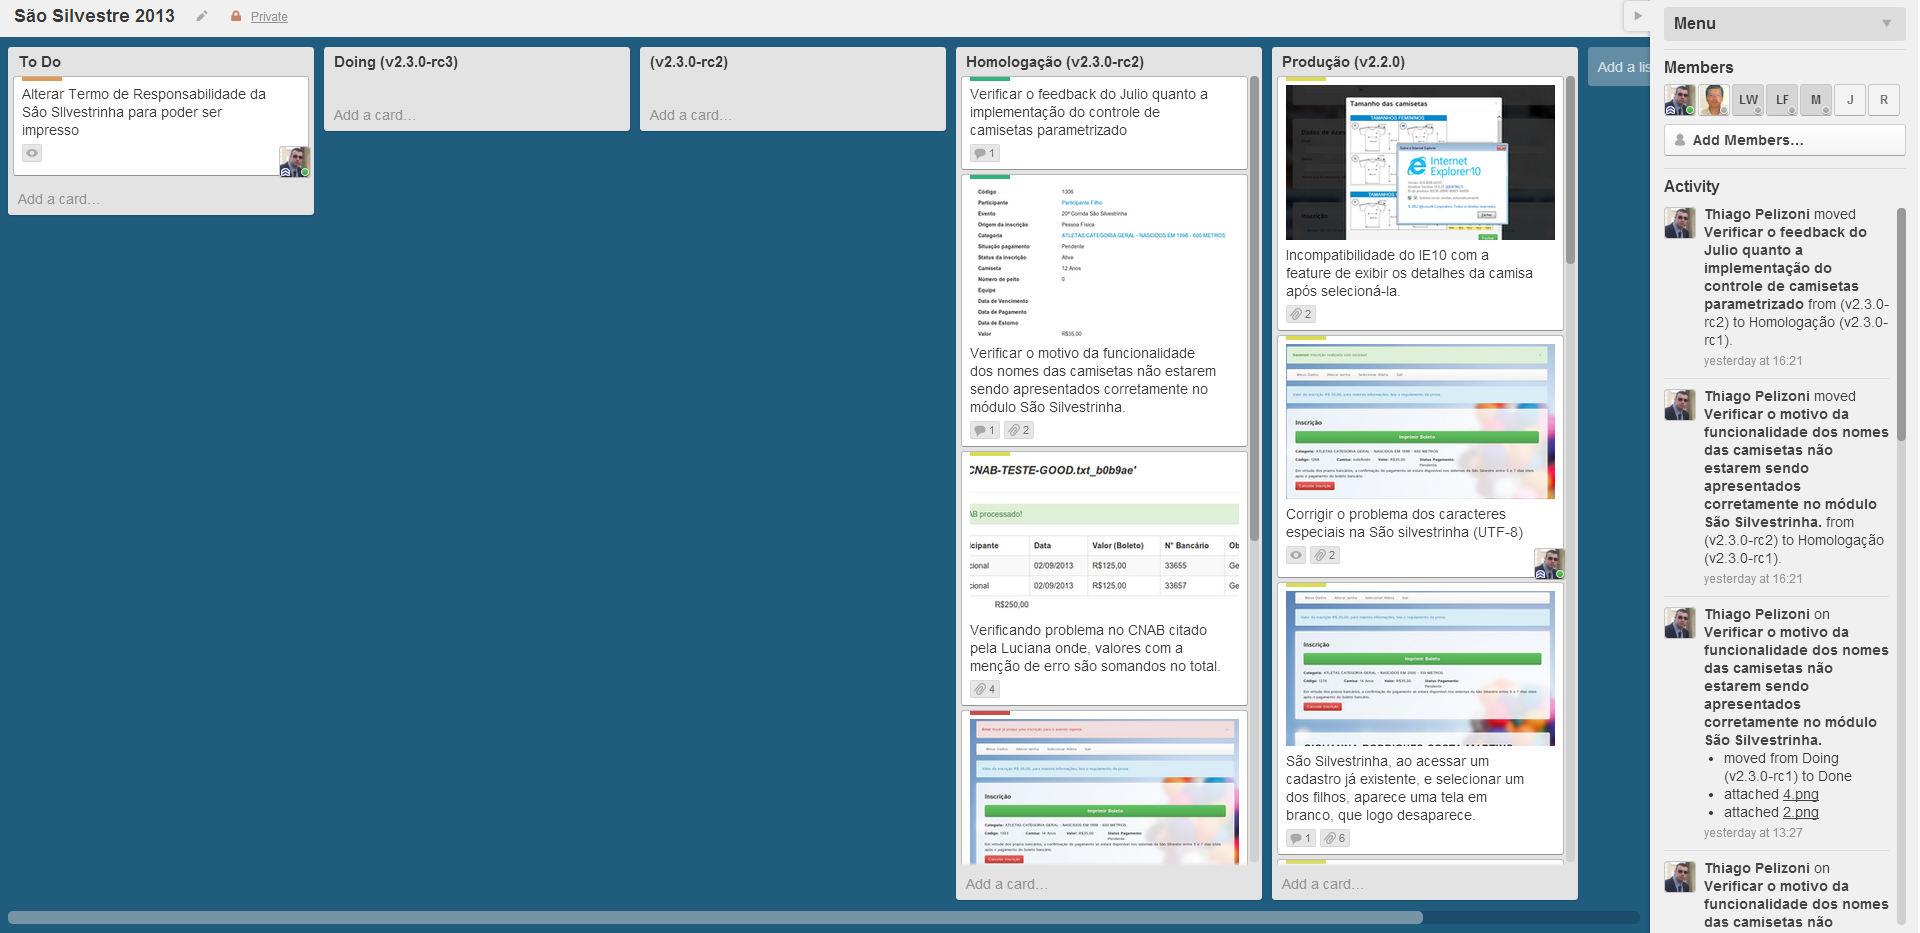
\includegraphics[width=160mm,height=90mm]{images/board.png}
\end{figure}

Cada coluna do board representa um estágio da tarefa onde, este board está dividido em cinco colunas, sendo elas:

\begin{itemize}
	\item \textit{To do}: Refere-se a todas as tarefas que necessitam ser feitas. Primeiras tarefas da coluna possuem maior prioridade.
	\item \textit{Doing}: Refere-se as tarefas que estão sendo feitas em um determinado momento. Cada programador pode ter apenas uma tarefa sendo feito em um dado momento. Quando algum item com maior prioridade, como por exemplo, um defeito em produção, o programador coloca sua tarefa novamente na coluna "To do", traz a tarefa que diz respeito ao problema para a coluna "Doing" e realiza a correção.
	\item \textit{Done}: Refere-se as tarefas que foram concluídas. Estas tarefas, após testadas pelo desenvolvedor e evidenciadas que estão de acordo com o especificado, estarão aptas para serem homologadas por quem solicitou tal tarefa.
	\item \textit{Homologação}: Referem-se as tarefas que encontram-se em ambiente de homologação sendo analizadas pelos solicitantes. Caso haja um problema, uma tarefa com o rótulo de "Correção" será criado na coluna "To do", e passará pelo processo descrito anteriormente. Caso as tarefas estejam de acordo, estas estarão áptas para irem para a produção.
	\item \textit{Produção}: Referem-se as tarefas que foram homologadas pelos solicitantes, geralmente, os analistas de negócios. Quando um problema em produção é encontrado, a tarefa criada faz referência a tarefa na coluna de produção, afim de manter um histórico.
\end{itemize}

\subsubsection{Tarefas}

Toda e qualquer nova tarefa, seja uma nova funcionalidade, alteração ou correção de bugs encontrados, independente do ambiente ao qual este se encontra, é gerado um card\footnote{Um card nada mais é do que uma tarefa dentro do board do Trello.} no Trello.

\begin{figure}[H]
  \caption{Uma tarefa do projeto}
  \centering 
  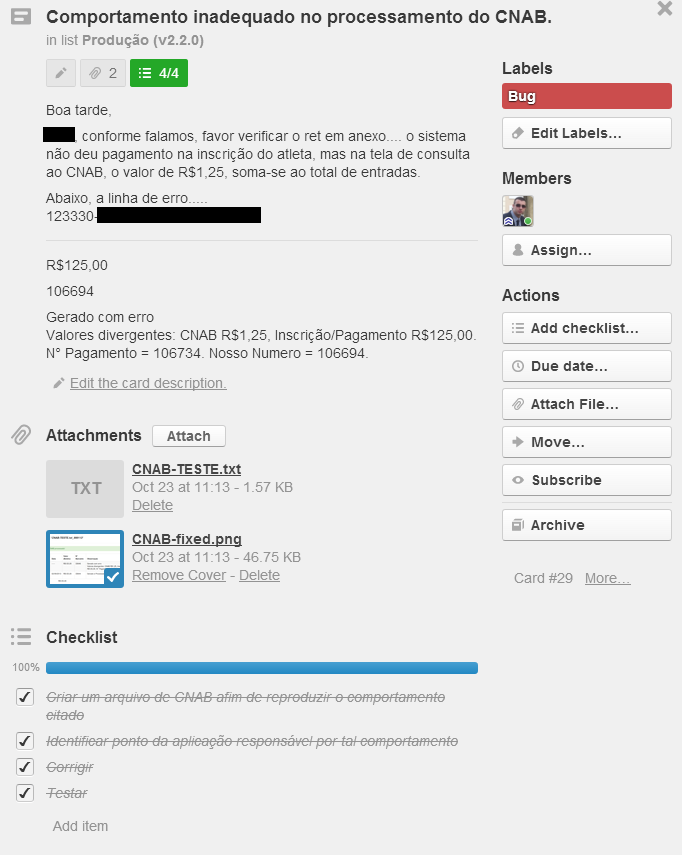
\includegraphics[width=150mm,height=180mm]{images/card.png}
\end{figure}

Como pode ser observado acima, uma tarefa segue uma estrutura básica:
\begin{itemize}
	\item \textit{Título}: Uma breve descrição da tarefa a ser realizada.
	\item \textit{Descrição}: Uma descrição detalhada da tarefa a ser realizada.
	\item \textit{Rótulo}: Qual é o tipo da tarefa.
	\item \textit{Membros}: Quem é o responsável por esta tarefa. Pode haver mais de uma pessoa dependendo do caso, por exemplo, um desenvolvedor e um analista de negócios.
	\item \textit{Checklist}: Quais os passos necessários para a conclusão da tarefa, afim de mensurar em quantos por cento esta atividade se encontra quando em execução.
	\item \textit{Anexos}: Evidências de que a funcionalidade ou as correções estão de acordo com o especificado. Em grande parte dos casos são screenshots.
\end{itemize}

\subsubsection{Rótulo para as tarefas}

Cada tarefa possui um rótulo, de modo a ficar mais fácil identificar o que cada tarefa é através de cores. Desta forma, ao olhar o board de modo geral, através dessas cores é possível identificar e reordenar as tarefas de acordo com sua prioridade de maneira mais fácil.

\begin{figure}[H]
  \caption{Rótulos das tarefas}
  \centering 
  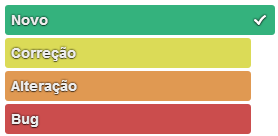
\includegraphics{images/labels.png}
\end{figure}

Como pode ser observado na imagem acima, atualmente, as tarefas podem ser de quatro tipos diferentes:

\begin{itemize}
	\item \textit{Novo}: Refere-se a alguma nova funcionalidade na aplicação.
	\item \textit{Correção}: Refere-se a correção de algum problema identificado no processo de homologação de uma funcionalidade, por exemplo, se uma funcionalidade foi implementada porém, ao verificá-la constatou-se um problema, um card com este rótulo será aberto para a devida correção.
	\item \textit{Alteração}: Refere-se a alteração de alguma funcionalidade na aplicação.
	\item \textit{Bug}: Refere-se a um problema encontrado em ambiente de produção. Geralmente estas tarefas em mais prioridade do que as demais.
\end{itemize}

\subsection{Indicadores}
Conforme descrito o processo de desenvolvimento onde, todas as informações referente ao projeto encontram-se na ferramenta Trello, será feita uma minuciosa investigação afim de levantar todos os defeitos

%%%%%%%%%%%%%%%%%%%%%%%%%%%%%%%%%%%%%%%%%%%%%%%%%%%%%%%%%%%%%%%%%%%%%%%%%%%%%%%%%%%
% 3. Resultados – o que foi observado?
%%%%%%%%%%%%%%%%%%%%%%%%%%%%%%%%%%%%%%%%%%%%%%%%%%%%%%%%%%%%%%%%%%%%%%%%%%%%%%%%%%%
\section{Resultados}
Resultados, o que foi observado

%%%%%%%%%%%%%%%%%%%%%%%%%%%%%%%%%%%%%%%%%%%%%%%%%%%%%%%%%%%%%%%%%%%%%%%%%%%%%%%%%%%
% 4. Considerações finais - o que se pode concluir dos resultados?
%%%%%%%%%%%%%%%%%%%%%%%%%%%%%%%%%%%%%%%%%%%%%%%%%%%%%%%%%%%%%%%%%%%%%%%%%%%%%%%%%%%
\section{Conclusão}
Considerações finais, o que se pode concluir dos resultados?

% Faz a criação das referências bibliográficas
\bibliography{Bibliografia}

\end{document}
